% to choose your degree
% please un-comment just one of the following
\documentclass[bsc,logo,frontabs,twoside,singlespacing,normalheadings,parskip]{infthesis}\usepackage[]{graphicx}\usepackage[]{color}
%% maxwidth is the original width if it is less than linewidth
%% otherwise use linewidth (to make sure the graphics do not exceed the margin)
\makeatletter
\def\maxwidth{ %
  \ifdim\Gin@nat@width>\linewidth
    \linewidth
  \else
    \Gin@nat@width
  \fi
}
\makeatother

\definecolor{fgcolor}{rgb}{0.345, 0.345, 0.345}
\newcommand{\hlnum}[1]{\textcolor[rgb]{0.686,0.059,0.569}{#1}}%
\newcommand{\hlstr}[1]{\textcolor[rgb]{0.192,0.494,0.8}{#1}}%
\newcommand{\hlcom}[1]{\textcolor[rgb]{0.678,0.584,0.686}{\textit{#1}}}%
\newcommand{\hlopt}[1]{\textcolor[rgb]{0,0,0}{#1}}%
\newcommand{\hlstd}[1]{\textcolor[rgb]{0.345,0.345,0.345}{#1}}%
\newcommand{\hlkwa}[1]{\textcolor[rgb]{0.161,0.373,0.58}{\textbf{#1}}}%
\newcommand{\hlkwb}[1]{\textcolor[rgb]{0.69,0.353,0.396}{#1}}%
\newcommand{\hlkwc}[1]{\textcolor[rgb]{0.333,0.667,0.333}{#1}}%
\newcommand{\hlkwd}[1]{\textcolor[rgb]{0.737,0.353,0.396}{\textbf{#1}}}%

\usepackage{framed}
\makeatletter
\newenvironment{kframe}{%
 \def\at@end@of@kframe{}%
 \ifinner\ifhmode%
  \def\at@end@of@kframe{\end{minipage}}%
  \begin{minipage}{\columnwidth}%
 \fi\fi%
 \def\FrameCommand##1{\hskip\@totalleftmargin \hskip-\fboxsep
 \colorbox{shadecolor}{##1}\hskip-\fboxsep
     % There is no \\@totalrightmargin, so:
     \hskip-\linewidth \hskip-\@totalleftmargin \hskip\columnwidth}%
 \MakeFramed {\advance\hsize-\width
   \@totalleftmargin\z@ \linewidth\hsize
   \@setminipage}}%
 {\par\unskip\endMakeFramed%
 \at@end@of@kframe}
\makeatother

\definecolor{shadecolor}{rgb}{.97, .97, .97}
\definecolor{messagecolor}{rgb}{0, 0, 0}
\definecolor{warningcolor}{rgb}{1, 0, 1}
\definecolor{errorcolor}{rgb}{1, 0, 0}
\newenvironment{knitrout}{}{} % an empty environment to be redefined in TeX

\usepackage{alltt}     % for BSc, BEng etc.
% \documentclass[minf,frontabs,twoside,singlespacing,parskip]{infthesis}  % for MInf

% APPENDIX
\usepackage[page]{appendix}

% FONT COMMANDS
\usepackage{fontspec}
\setmainfont[Mapping=tex-text,Numbers=OldStyle]{fbb}
\setsansfont[Mapping=tex-text,Numbers=OldStyle,Scale=MatchLowercase]{Gill Sans}
\setmonofont[Mapping=tex-text,Scale=MatchLowercase]{Inconsolata}


% DISPLAY TODOS
%\usepackage[disable]{todonotes}
\usepackage[draft,bordercolor=white,backgroundcolor=yellow!60,linecolor=black,colorinlistoftodos]{todonotes}

% MAKE SURE TODOS ARE INLINE
\let\Oldtodo\todo
\renewcommand{\todo}[1]{\Oldtodo[inline]{#1}}

% INCLUDE CODE FILES
\usepackage{minted}

% ALLOW TWO FIGURES NEXT TO EACH OTHER
\usepackage{subcaption}


% ENSURE CHAPTERS WORK IN PDF VIEWERS
\usepackage[]{hyperref}
\hypersetup{
    pdftitle={Storm on Multi-core},
    pdfauthor={Mark Nemec},
    %pdfsubject={Your subject here},
    %pdfkeywords={keyword1, keyword2},
    bookmarksnumbered=true,
    bookmarksopen=true,
    bookmarksopenlevel=1,
    %colorlinks=true,
    pdfstartview=Fit,
    pdfpagemode=UseOutlines,
    pdfpagelayout=TwoPageRight
}
\IfFileExists{upquote.sty}{\usepackage{upquote}}{}
\begin{document}

\title{Storm on Multi-core}
\author{Mark Nemec}
\course{Computer Science}
\project{4th Year Project Report}

\date{\today}

\abstract{This is the abstract.}

\maketitle

\section*{Acknowledgements}
Acknowledgements go here.

\tableofcontents
\listoflistings

\pagenumbering{arabic}

\chapter{Introduction}

\section{Motivation}

In recent years, there has been an explosion of cloud computing software. After Google published their paper on MapReduce \citep{dean2010mapreduce}, many new open-source frameworks for distributed computation have emerged, most notably Apache Hadoop \citep{ApacheHadoop} for batch processing and Apache Storm \citep{ApacheStorm} for real-time data stream processing.

The main idea of these frameworks is to split the work that needs to be carried out and distribute it across nodes of a cluster. Commercial companies and researchers have been able to utilise these frameworks and create distributed systems which can accomplish things that would not be otherwise possible. This has mostly been allowed by the low price and good horizontal scaling properties of commodity hardware.

\todo{Quote that they are standard.}

At the same time, chip makers have been increasing the number of cores in processors and now we are at a point where servers with 10-core processors are standard. Moreover, most high-end servers support multiple processor sockets thus furthering the parallelisation possible with a single machine even more.

The price of multi-core servers has been going down as well. In 2008, a typical Hadoop node had two dual-core processors and 4 GB of random access memory (RAM). Nowadays, a server with two eight-core processors and 256 GB of RAM can be purchased for roughly \$10,000 USD \citep{Kumar:2013:HSD:2536274.2536314}. Hence a single server today might have better processing power than a small cluster from a few years ago \citep{Kumar:2013:HSD:2536274.2536314}.

% TODO: Here talk about What this paper is about !
% TODO: Maybe mention the Hadoop multi-core paper
% TODO: Maybe a section - move main idea here?
This project is about taking the ideas from the distributed system Apache Storm and applying them in the context of multi-core instead of clusters.

%% TODO: After that comes Motivation which explains why it's a good idea!

While the cost of a commodity hardware cluster might be lower than the price of a single computer with equal power there are certain limitations:

\begin{itemize}

\item The nodes of a cluster communicate through network. This limits the speed of communication between processes that live on different nodes.

\item Distributed systems waste resources by replicating data to ensure reliability.

% TODO: Maybe mention renting vs owning here
\item Running a distributed computation on commodity hardware usually requires a data centre or renting out instances on cloud computing services such as Amazon EC2 or Rackspace. This is not ideal for some use cases which require full control over the system or a heightened level of security. 

\end{itemize}

On the other hand, even though Moore’s law still holds true, processor makers now favour increasing the number of cores in CPU chips to increasing their frequency. This trend implies that the “free lunch” of getting better software performance by upgrading the processor is over and programmers now have to design systems with parallel architectures in mind. However, there are some limitations to this as well:

\begin{itemize}

\item It is generally believed that writing parallel software is hard. The traditional techniques of message passing and parallel threads sharing memory require the programmer to manage the concurrency at a fairly low level, either by using messages or locks.

%% TODO: Rephrase "nice if they could"
\item Apache Storm has become the de facto tool used in stream processing on a cluster and according to their "Powered By" page \cite{Anonymous:eikzOt4-} there are tens of companies already using Storm to process their real-time streams. It would be nice if they could keep that code.

\end{itemize}

\section{Main Idea}

The solution proposed in this report is to take the existing Apache Storm project and port it to multi-core. This is implemented in Storm-MC - a library with an API compatible with Apache Storm. This allows programmers to take an existing application written with Apache Storm in mind and run it on multi-core. This way, we can avoid network latency and enjoy the significant performance improvements of a shared-memory environment.

\section{Structure of the Report}

The remainder of the report is structured as follows:

\begin{itemize}
	\item \textbf{Chapter 2} presents an overview of related literature and gives background on data stream processing and multi-core architectures.
	\item \textbf{Chapter 3} explains the concepts used in Apache Storm as well as the architecture of a Storm cluster.
	\item \textbf{Chapter 4} describes how Apache Storm was ported over to Storm-MC.
	\item \textbf{Chapter 5} gives an overview the implementation details of Storm-MC.
	\item \textbf{Chapter 6} discusses the evaluation results of Storm-MC.
	\item \textbf{Chapter 7} presents the conclusion of this report.
\end{itemize}


%\chapter{Prior Work}



\chapter{Background}

In this chapter we give background information necessary to understand the design of Storm-MC. We give a quick overview of Apache Storm \ref{sec:storm_overview}, explain the concepts (\ref{sec:concepts}) used in Storm, show an example Storm program (\ref{sec:example_topology}), give details about the underlying architecture of Storm (\ref{sec:storm_arch}), and finally  describe the serialisation used by Storm.

\section{Storm Overview}
\label{sec:storm_overview}

Apache Storm was developed in a mix of Java and Clojure. As mentioned by the author of Storm in \cite{Marz_2014}, writing the Storm interfaces in Java ensured large potential user-base while writing the implementation in Clojure increased productivity.

To ensure API compatibility with Storm, Storm-MC was developed using the same set of languages. This allowed for code reuse and not having to re-implement functionality already present in Storm. Hence, in the following sections we describe Storm in greater detail in hope that this will later clarify design choices made for Storm-MC.

\section{Storm Concepts}
\label{sec:concepts}

\subsection{Core Concepts}

There are several core concepts used by Storm and hence by extension Storm-MC as well. These concepts are put together to form a simple API that allows the user to break down a computation into separate components and define how these components interact with each other. The three core concepts of Storm are:

\begin{description}
  \item[Spout] \hfill \\
  A spout is a component that represents the source of a data-stream. Typically, a spout reads from a message broker such as RabbitMQ \cite{RabbitMQ} or Apache Kafka \cite{ApacheKafka} but can also generate its own stream or read from somewhere like the Twitter streaming API.
  \item[Bolt] \hfill \\
  A bolt is a component that transforms tuples from its input data stream and emits them to its output data stream. A bolt can perform a range of functions e.g. filter out tuples based on some criteria or perform a join of two different input streams.
  \item[Topology] \hfill \\
  The programmer connects spouts and bolts in a directed graph called topology which describes how the components interact with each other. The topology is then submitted to Storm for execution.
\end{description}

\subsection{Additional Concepts}

\begin{description}
  \item[Stream] \hfill \\
  A stream is defined as an unbounded sequence of tuples. Streams can be thought of as edges of a topology connecting bolts and spouts (vertices).
  \item[Tuple] \hfill \\
  A tuple wraps named fields and their values. The values of fields can be of different types. When a component emits a tuple to a stream it sends that tuple to every bolt subscribed to the stream.
  \item[Stream Grouping] \hfill \\
  Every bolt needs to have a type of stream grouping associated with it. This grouping decides the means of distributing the tuples coming from the bolt's input streams amongst the instances of the bolt task. Following are the possible types of stream grouping:
  \begin{description}
  	\item[Shuffle] Randomly partitions the tuples among all the bolt tasks.
  	\item[Fields] Hashes on a subset of the tuple fields.
  	\item[All] Replicates the entire stream to all the bolt tasks.
  	\item[Direct] The producer of the tuple decides which task of the bolt will receive this tuple.
  	\item[Global] Sends the entire stream to a single bolt task.
  	\item[Local or Shuffle] Prefers sending to executors in the same worker process, if that is not possible it uses the same strategy as shuffle.
  \end{description}
\end{description}

Users are also able to specify their own custom grouping by implementing the \texttt{CustomStreamGrouping} interface.

All the components of a Storm topology execute in parallel. The user can specify how much parallelism he wants associated with every component and Storm spawns the necessary number of threads. This is done through a configuration file, defined in YAML, which is submitted along with the topology.

There are two additional bolts running for every topology:

\begin{description}
	\item[Acker] \hfill \\
	The Acker bolt guarantees fault tolerance for the topology. It tracks every tuple that was produced and ensures that the tuple has been acknowledged by every bolt of the stream.
	\item[System Bolt] \hfill \\
	The System bolt is useful in two ways:
	\begin{description}
		\item[Metrics] System bolt collects metrics on the local Java Virtual Machine (JVM). Other components can subscribe to these metrics and receive their values at  regular intervals.
		\item[Ticks] Components of a topology can subscribe to receive tick tuples in regular intervals. These tuples can be used to trigger some event of a component.
	\end{description}
\end{description}

\section{Example Topology}
\label{sec:example_topology}

\begin{figure}[!htb]
	\centering
	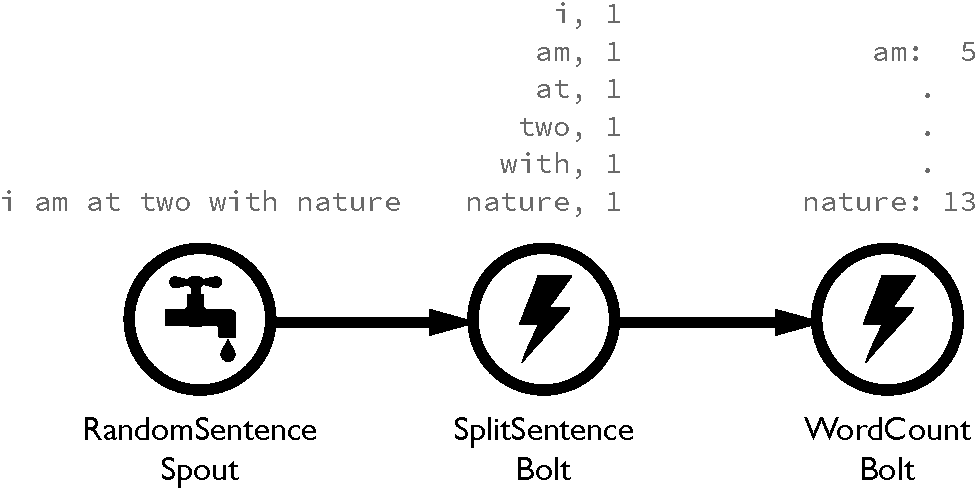
\includegraphics[scale=0.7]{pdf/wordcount_topology.pdf}
	\caption{WordCount topology.}
	\label{fig:wordcount_topology}
\end{figure}

A classic example used to explain Storm topologies is the WordCount topology. In this topology, there is a spout generating random sentences, a bolt splitting the sentences on white space, and a bolt counting occurrences of every word. Figure \ref{fig:wordcount_topology} shows how we could represent this topology graphically.

This may seem as a simplistic example but it is useful when demonstrating how easy it is to implement a working topology using the Storm API.

\begin{listing}[!htb]
\inputminted{java}{code/WordCountTopology.java}
\caption{WordCountTopology.java}
\label{listing:wordcount_topology}
\end{listing}

Listing \ref{listing:wordcount_topology} shows how the topology is put together to form a graph of components. Storm uses the Builder design pattern to build up the topology which is then submitted to Storm for execution. The last argument to the setBolt/setSpout method is the number of parallel tasks we want Storm to execute for the respective component. For implementation of the spout and bolts used in this topology, refer to appendix \ref{ch:listings}.

\section{Storm Architecture}
\label{sec:storm_arch}

\begin{figure}[!htb]
	\centering
	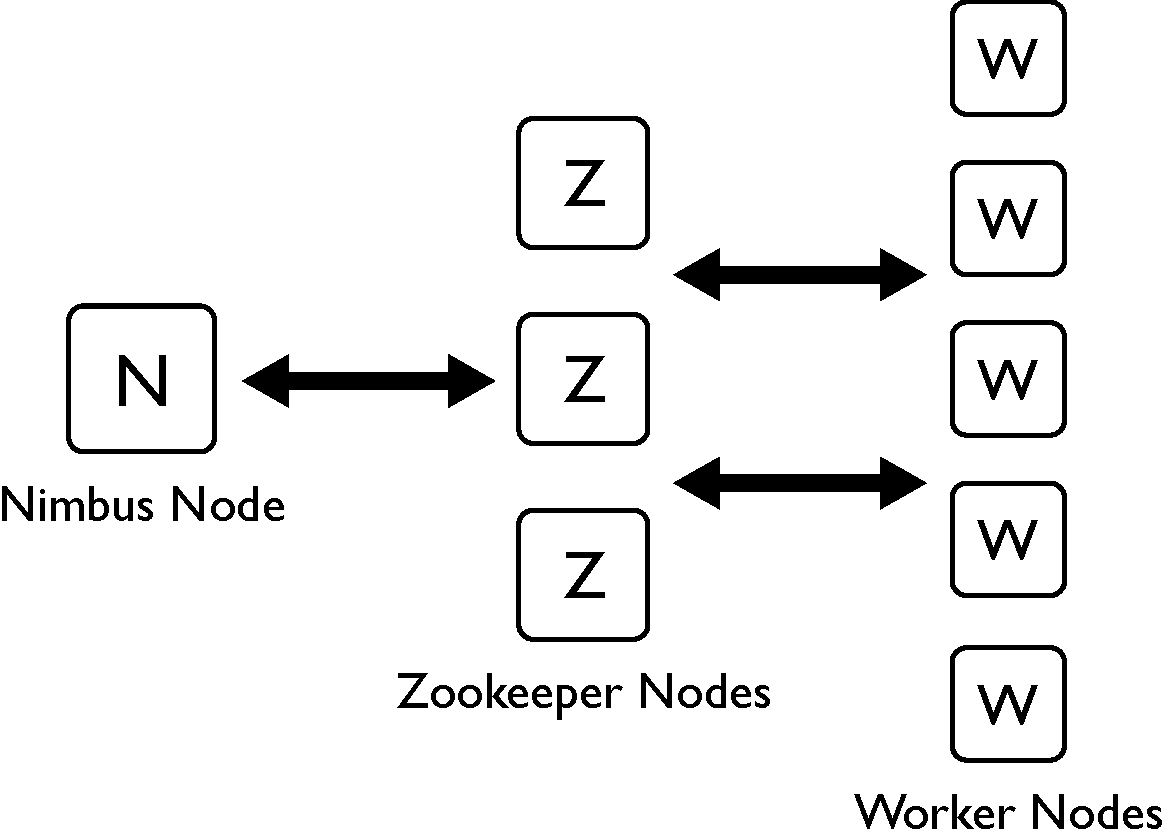
\includegraphics[scale=0.5]{pdf/storm_arch.pdf}
	\caption{Apache Storm Architecture.}
	\label{fig:storm_arch}
\end{figure}

%\todo{Maybe highlight similarities to Hadoop}

A Storm cluster adopts the Master-Worker pattern. To set up a Storm topology, the user launches daemon processes on nodes of the cluster and submits the topology to the master node, also called Nimbus. The worker nodes receive task assignments from the master and execute on them. The coordination between the master node and the worker nodes is handled by nodes running Apache Zookeeper \cite{ApacheZookeeper}. Figure \ref{fig:storm_arch} shows a graphical representation of Storm Architecture.

\subsection{Nimbus Node}

The master node runs a server daemon called Nimbus. The main role of Nimbus is to receive topology submissions from clients. Upon receiving a topology submission, Nimbus takes the following steps:

\begin{description}
	\item[Validate the topology] \hfill \\
	The topology is validated using a validator to ensure that the submitted topology is valid before trying to execute it. The user can implement his own validator or use the default validator provided by Storm.
	\item[Distribute the topology source code] \hfill \\
	Nimbus ensures that the workers involved in the topology computation have the source code by sending it over the network.
	\item[Schedule the topology] \hfill \\
	Nimbus runs a scheduler that distributes the work among workers of the cluster. Similarly to validation, the user can implement his own scheduler or use the default scheduler provided by Storm. The default scheduler uses a simple Round-robin strategy.
	\item[Activate the topology] \hfill \\
	Nimbus transitions the topology to active state which tells the worker nodes to start executing it.
	\item[Monitor the topology] \hfill \\
	Nimbus continues to monitor the topology by reading heartbeats sent by the worker nodes to ensure that the topology is executing as expected and worker nodes have not failed.
\end{description}


Nimbus is an Apache Thrift \cite{ApacheThrift} service (more on Thrift in section \ref{sec:serialisation}) that listens to commands submitted by clients and modifies the state of a cluster accordingly. Following are the commands supported by Nimbus:

\begin{description}
	\item[Submit a topology] \hfill \\
	Clients can submit a topology defined in a Java Archive (JAR) file. The Nimbus service then ensures that the topology configuration and resources are distributed across the cluster and starts executing the topology.
	\item[Kill a topology] \hfill \\
	Nimbus can stop running a topology and remove it from the cluster. The cluster can still continue executing other topologies.
	\item[Activate/deactivate a topology] \hfill \\
	Topologies can be deactivated and reactivated by Nimbus. This could be useful if the spout temporarily cannot produce a stream and the user does not want the cluster to execute idly.
	\item[Rebalance a topology] \hfill \\
	Nimbus can rebalance a topology across more nodes. Thus if the number of nodes in the cluster changes the user can increase or decrease the number of nodes involved in the topology.
\end{description}

%\todo{Is listing this really necessary?}

\subsection{Worker Nodes}

The worker nodes run a daemon called Supervisor. There are 4 layers of abstraction which control the parallelism of a worker node.

\begin{description}
	\item[Supervisor] \hfill \\
	A supervisor is a daemon process the user runs on a worker node to make it part of the cluster. It launches worker processes and assigns them a port they can receive messages on. Furthermore, it monitors the worker processes and restarts them if they fail. A worker node runs only one supervisor process.
	\item[Worker] \hfill \\
	A worker process is assigned a port and listens to tuple messages on a socket associated with the port. A worker launches executor threads as required by the topology. Whenever it receives a tuple, it puts it on a queue where it is picked up by one or more executors of the worker process.
	
	Furthermore, the worker has a transfer queue where its executors enqueue tuples ready to be sent downstream. There can be multiple workers processes running inside one supervisor.
	\item[Executor] \hfill \\
	An executor controls the parallelism within a worker process. Every executor runs in a separate thread. An executor's job is to pick up tuples from the receiver queue of the worker, perform the task of a component it represents, and put the transformed tuples on the transfer queue of the worker. There can be many executors running inside one worker and an executor performs one (the usual case) or more tasks.
	\item[Task] \hfill \\
	A task represents the actual tuple processing function. However, within an executor thread all the tasks are executed sequentially. The main reason for having tasks is that the number of tasks stays the same throughout the lifetime of a topology but the number of executors can change (by rebalancing). Thus if some worker nodes in the cluster go down, the topology can continue executing with the same number of tasks as before.
\end{description}

\subsection{Zookeeper Nodes}
\label{subsec:zookeeper}

The Storm cluster contains a number of Zookeeper nodes which coordinate the communication between the master and the workers. Storm does this by storing the state of the cluster on the Zookeper nodes where both Nimbus and worker nodes can access it.

The cluster state contains worker assignments, information about topologies, and heartbeats sent by the worker nodes back to Nimbus. Apart from the cluster state, Storm is completely stateless. Hence, if the master node or a worker node fail the cluster continues executing. The only time the cluster stops executing is if all the Zookeper nodes die.

\section{Serialisation}
\label{sec:serialisation}

Since Storm topologies execute on a cluster all components need to be serialisable. This is achieved with Apache Thrift. Components are defined as Thrift objects and Thrift generates all the Java serialisation code automatically.

Furthermore, since Nimbus is a Thrift service Thrift generates all the code required for remote procedure call (RPC) support. This allows defining topologies in any of the languages supported by Thrift and easy cross-language communication with the Nimbus service.


\chapter{Bringing Storm to Multi-core}

The following chapter explains the design of Storm-MC. We describe how Apache Storm behaves on multi-core machines (\ref{sec:storm_on_mc}), how the Storm architecture was ported over to multi-core (\ref{sec:storm_mc_arch}), and we list feature differences between Apache Storm and Storm-MC (\ref{sec:differences}).

\section{Apache Storm on Multi-core}
\label{sec:storm_on_mc}

To begin, we discuss why Apache Storm does not perform optimally on a single multi-core machine. Storm can be ran in local mode where it emulates execution on a cluster. This mode exists so that it is possible to debug and develop topologies without needing access to a cluster. However, there are several reasons why the local mode is not as performant as it could be.

\subsection{Tuple Processing Overhead}

\begin{figure}[!htb]
	\centering
	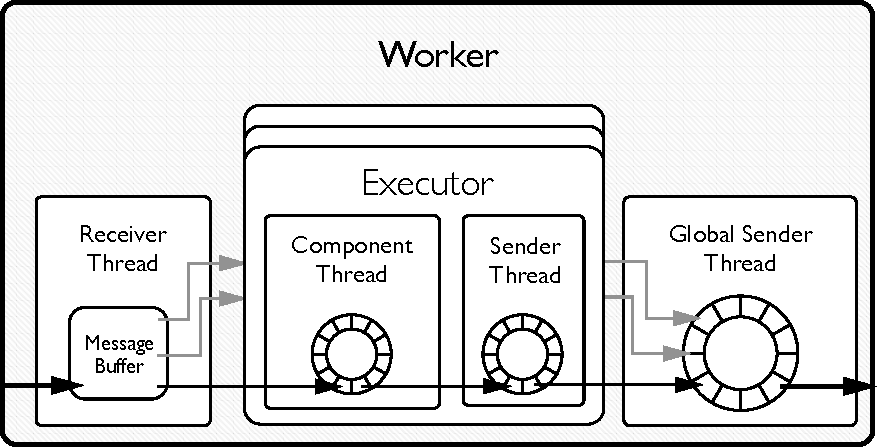
\includegraphics[scale=0.7]{pdf/worker_inside.pdf}
	\caption{Tuple processing in Apache Storm.}
	\label{fig:worker_inside}
\end{figure}

Figure \ref{fig:worker_inside} shows how tuple processing is implemented inside a Storm worker process. The tuple is read from a message buffer by the receiver thread of the worker and put on a receive queue of the target executor. The tuple is then picked up by the component thread of the executor for task execution.

After the component thread has executed the task it puts the tuple on the executor send queue. There, it is picked up by the executor sender thread which puts the tuple on the global send queue of the worker. Lastly, the global sender thread of the worker serialises the tuple and sends it downstream.

Alternatively, if the tuple is forwarded to an executor in the same worker process it is put on the receive queue of the corresponding executor directly after task execution.

The queues used in Storm are implemented as ring buffers using the LMAX Disruptor library \citep{LMAXDisruptor}. Detailed background on how Disruptor works and its performance benchmarks can be found in \citep{Thompson_Farley_Barker_Gee_Stewart_2011}.

There is significant overhead required to simulate sending tuples to executors in other worker nodes. For one, there is the overhead from the tuple passing through the three queues of a worker. The authors of LMAX Disruptor showed that a three step pipeline has half the throughput of a single consumer-producer pipeline \citep{DisruptorWiki}.

Furthermore, to emulate over-the-network messages Storm uses a \texttt{Hashmap} of \texttt{LinkedBlockingQueue}s which according to \cite{Thompson_Farley_Barker_Gee_Stewart_2011} has several orders of magnitude lower performance than the Disruptor. Due to less write contention, lower concurrency overhead, and being more cache-friendly the Disruptor pattern can offer latency of inter-thread messages lower than 50 nanoseconds and a throughput of over 25 million messages per second.

\subsection{Thread Overhead}

\todo{Maybe mention waiting strategies?}

\begin{description}
	\item[Acker Bolt] \hfill \\
	The Acker is included in every topology. The Acker bolt can be disabled via the configuration file. In such a case it is mostly idle since it does not receive any messages but it can still use up resources especially if it waits for messages using a busy waiting strategy.
	\item[Heartbeats \& Timers] \hfill \\
	Every worker has a heartbeat thread that simulates sending heartbeat messages to the Nimbus node. It does this by writing to a local cache which is persisted to a file by a write on every heartbeat. Since the write is implemented using the \texttt{java.io} package the write is blocking i.e. the thread cannot continue until the write is completed. While heartbeats are essential in cluster mode to signal the node being alive, there is no need for them in local mode.
	\item[Zookeeper Emulation] \hfill \\
	More overhead is produced by a local Zookeper server which emulates the Zookeeper nodes of a cluster. Running the Zookeeper server is a massive addition to the list of overheads as shown in the following paragraphs. The purpose of Zookeeper is to maintain states of running topologies and nodes of the cluster. As we will show in the following sections maintaining this state on multi-core is not necessary.
\end{description}

During profiling we found that a topology with one worker and three executors was being executed with 55 threads (not including system JVM threads and threads created by the profiler). Table \ref{table:breakdown} shows a breakdown of what the individual threads were used for.

\begin{table}[h!]
\centering
\begin{tabular}{@{}lc@{}}
    \textbf{Spout Parallelism} & \textbf{\# of Threads} \\ \toprule
    Main Thread & 1  \\
	Worker Sender \& Receiver Threads & 2  \\
    Acker \& System Component Threads & 2  \\
    Executor Component Threads & 3  \\
    Executor Sender Threads & 5  \\
    Various Timers \& Event Loops & 14  \\
    Zookeper Server & 28  \\
\end{tabular}
\caption{Breakdown of threads used by Storm to execute a 3-component topology.}
\label{table:breakdown}
\end{table}

To find out what state the threads were actually in at any given time the topology was executed for three minutes and a JVM thread dump was recorded every second. The average results of this experiment can be observed in table \ref{table:dump} and the state distribution over time can be seen in figure \ref{fig:dump-plot}.

\begin{table}[h!]
\centering
\begin{tabular}{@{}lc@{}}
    \textbf{Spout Parallelism} & \textbf{\# of Threads} \\ \toprule
    RUNNABLE & 8  \\
	TIMED WAITING & 22  \\
    WAITING & 25  \\
\end{tabular}
\caption{Average number of recorded thread states over a three minute period.}
\label{table:dump}
\end{table}

<<dump-plot, echo=FALSE, cache=TRUE, fig.cap="Thread state distribution over time.", fig.height=3>>=
@

Even though three minutes may seem to be a very short amount of time the fact that there is almost no variation shows that it is sufficient. As can be seen from the table, most of the threads were either in state \texttt{WAITING} or \texttt{TIMED WAITING}. According to the Java documentation on thread states \citep{JavaThreads} these two states are used for threads that are waiting for an action from a different thread and cannot be scheduled by the scheduler until that action is executed.

On average there were eight threads in state \texttt{RUNNABLE} which JVM uses to mark threads which are executing on the JVM and are possibly waiting for resources from the operating system (OS) such as processor \citep{JavaThreads}. Hence, these are threads directly competing to be scheduled by the OS. This means that for three components running in parallel there are five threads doing potentially unnecessary work.

In the subsequent sections we will show that these threads were in fact unnecessary and we will discuss how the number of threads was reduced. In fact, to execute the same topology on Storm-MC requires only 5 threads.

\section{Storm-MC Design}
\label{sec:storm_mc_arch}

The design we adopted for porting worker nodes is to only have one worker process running all the executor threads of a topology.

Additionally, the code for the Nimbus service was merged with the worker. This was done because there is no need to run Nimbus and worker specific code at the same time. Once Nimbus sets up the topology, all the work is done by the worker. Hence they can be executed serially.

\subsection{Nimbus}

Unlike Nimbus executing on a Storm cluster, Nimbus in Storm-MC does not support running multiple topologies at the same time. However, to do that one only needs to run the topology in a separate process. This is because unlike when executing on the cluster different topologies do not need to share any state and it is more natural to execute them as separate processes.

This has the added benefit of each process having its own part of main memory thus reducing cache conflicts as shown in \citep{Chandra:2005:PIC:1042442.1043432} and providing higher security by not having different topologies share memory space. Additionally, if a single thread of one topology is blocking it does not block other topologies.

Nimbus on Storm-MC does not support scheduling topologies. Since within one process there is only one topology running at a time and the hardware configuration of the machine does not change, the parallelism is clearly defined by the number of executors per component specified in the topology configuration.

One way to implement scheduling could be to pin threads to specific cores. Unfortunately, Java does not provide support for CPU affinity, the assignments are handled automatically by the JVM. Potentially, this could be achieved by using C or C++, both of which support CPU affinity, but this was not implemented in Storm-MC.

The role of Nimbus in Storm-MC has effectively been reduced to validating the topology and passing it along to the worker part of the process which handles the topology execution.

\subsection{Worker}

In Apache Storm, a worker node runs the supervisor daemon, which in turns launches worker processes which contain executor threads which contain tasks. In Storm-MC, however, there is only one worker process which contains all the executor threads and their tasks.

This design has several benefits:

\begin{itemize}
	\item All the inter-thread communication is occurring within one worker process.
	\item Supervisor can be removed as there is no need to synchronise multiple workers.
	\item There is no need to simulate over-the-network message passing.
	\item Message passing between executor threads within a worker stays the same as in Apache Storm.
\end{itemize}

The role of worker is to launch executors and provide them with a shared context through which they can communicate. This is done by via a map of executor identifiers to Disruptor queues which the executors use to pass tuples between each other.

A comparison of an Apache Storm worker node and its Storm-MC equivalent is depicted in figure \ref{fig:comparison}.

\begin{figure}[!htb]
\centering
\begin{subfigure}{.5\textwidth}
  \centering
  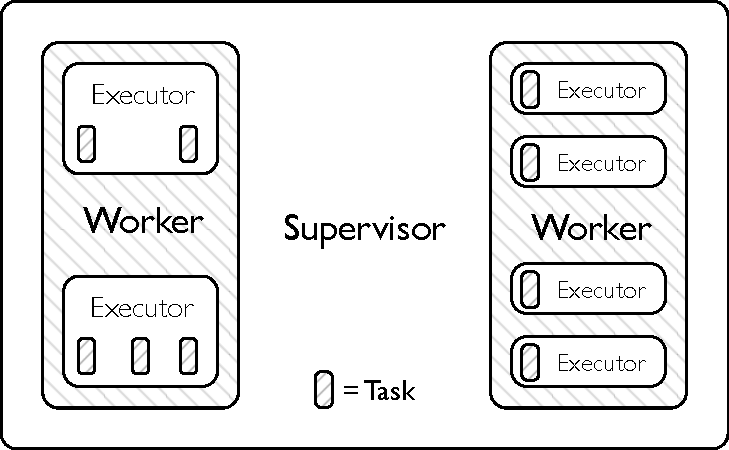
\includegraphics[width=0.95\linewidth]{pdf/distributed_worker.pdf}
  \caption{Worker node in Apache Storm.}
  \label{fig:comparison1}
\end{subfigure}%
\begin{subfigure}{.5\textwidth}
  \centering
  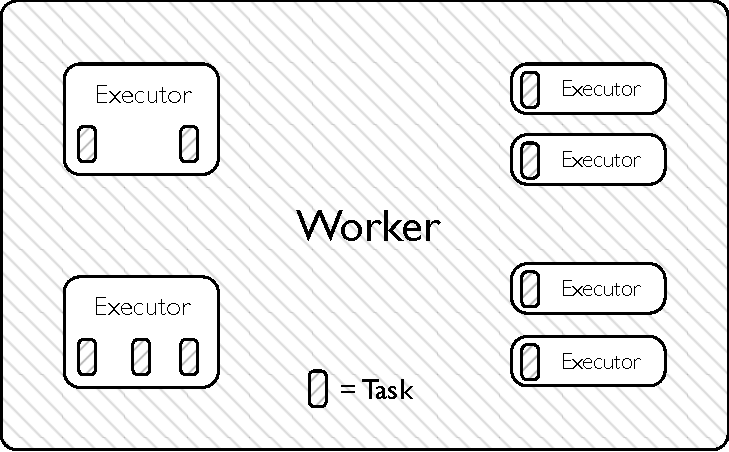
\includegraphics[width=0.95\linewidth]{pdf/local_worker.pdf}
  \caption{Worker node equivalent in Storm-MC.}
  \label{fig:comparison2}
\end{subfigure}
\caption{Comparison of a worker in Storm and Storm-MC}
\label{fig:comparison}
\end{figure}

\subsection{State}

As mentioned before, Storm-MC is completely stateless. The cluster state that was managed by Zookeeper in Apache Storm was completely stripped away. This state was only relevant when multiple topologies were sharing resources.

\subsection{Serialisation}

Great amount of work was put into removing the dependency of Storm-MC on Apache Thrift. This was done not only for optimisation purposes but also to reduce code bloat and remove an unnecessary dependency since there is no serialisation required in multi-core communication.

%This required refactoring all the data types generated by Thrift used all over the codebase. This significantly reduced the size of the codebase and made the code more readable and self-documenting than the code generated by Thrift.


\todo{Mention overhead by running SystemBolt vs just timer in Storm-MC}

%\subsection{Metrics}
%
%The metrics API was ported over from Apache Storm. However, there are several differences 

\subsection{Tuple Processing}

\begin{figure}[!htb]
	\centering
	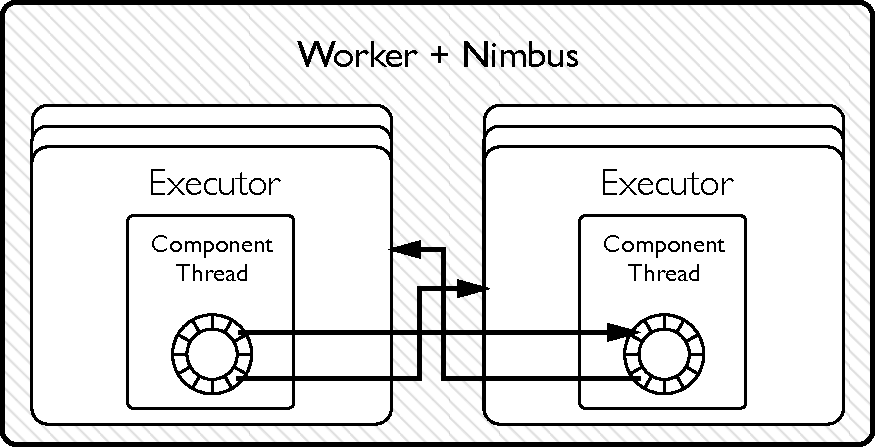
\includegraphics[scale=0.7]{pdf/worker_inside_mc.pdf}
	\caption{Tuple processing in Storm-MC.}
	\label{fig:worker_inside_mc}
\end{figure}

The implementation of tuple processing in Storm-MC is depicted in figure \ref{fig:worker_inside_mc}. As can be seen from the figure, the queues used for remote message sending were stripped away and there is only one Disruptor queue for every executor. Once an executor is done processing a tuple it simply puts it on the Disruptor queue of its downstream bolts.

Thus the tuple processing in Storm-MC is a variant of multiple producer single consumer problem. We considered several other options such as \texttt{ArrayBlockingQueue} when implementing the tuple processing mechanism. However, the Disruptor shows superior throughput and latency compared to alternative solutions \citep{DisruptorWiki}.

\section{Differences between Apache Storm and Storm-MC}
\label{sec:differences}

\begin{table}[h!]
\centering
\begin{tabular}{@{}lcc@{}}
    \textbf{Feature} & \textbf{Apache Storm} & \textbf{Storm-MC} \\ \toprule
    Multiple Topologies & \cmark & \xmark \\
	Trident Support & \cmark & \xmark \\
    Built-in Metrics & \cmark & \xmark \\
    Nimbus as a Server & \cmark & \xmark \\
    Multi-language Topologies & \cmark & \cmark \\
    Hooks & \cmark & \cmark \\
    Metrics & \cmark & \cmark \\
    Tick Tuples & \cmark & \cmark \\
\end{tabular}
\caption{Feature comparison of Apache Storm and Storm-MC.}
\label{table:features}
\end{table}


\chapter{Evaluation}

In this chapter we evaluate Storm-MC. We do this by comparing its performance against the local mode of Apache Storm.

\section{Performance}

\subsection{Software Setup}

\todo{Change versions below as applicable. Link to GitHub for source?}

All performance benchmarks were ran using the following software packages:

\begin{itemize}
	\item Apache Storm version 0.9.2
	\item Storm-MC version 0.1.5
	\item A fork of IBM Storm Email Benchmarks version 0.1.4
	\item Storm-benchmark version 0.1.0
\end{itemize}

The Apache Storm source code had to be adapted to include a workaround for a deadlock bug present in version 0.9.2. This bug caused a topology to exit with threads left in Zombie state under certain conditions. This prevented Storm from logging the benchmark metrics after execution.

Version 0.1.5 is the latest version of Storm-MC as of this moment. The first release was version 0.1.0 which was production-ready but since then there were 5 minor versions fixing bugs as they were discovered during testing.

IBM open sourced a suite of benchmarks which they used to compare Apache Storm to their real-time stream system IBM Infosphere Streams. These benchmarks were adapted and used to benchmark Apache Storm and Storm-MC.

Lastly, a number of spout and bolt components were used from the storm-benchmark project which Apache Storm developers use to benchmark Storm.

Since Storm-MC reuses package names from Apache Storm, the same benchmark is directly executable by both libraries. This saved a lot of time and furthermore there is no need to maintain two benchmarks suites.

\todo{Go into more detail which components were re-used and where?}

\subsection{Hardware Setup}

The benchmarks were executed on the following hardware:

\todo{This is currently student.compute, find out what it is.}

\subsection{WordCount Topology}

The first topology we tested for performance is a variant of the aforementioned WordCount topology. Recall, that this topology is shown graphically on figure \ref{fig:wordcount_topology}. The topology was ran with 3 executors running for every component.

This topology is considered to be CPU-intensive.



\begin{knitrout}
\definecolor{shadecolor}{rgb}{0.969, 0.969, 0.969}\color{fgcolor}\begin{figure}

{\centering 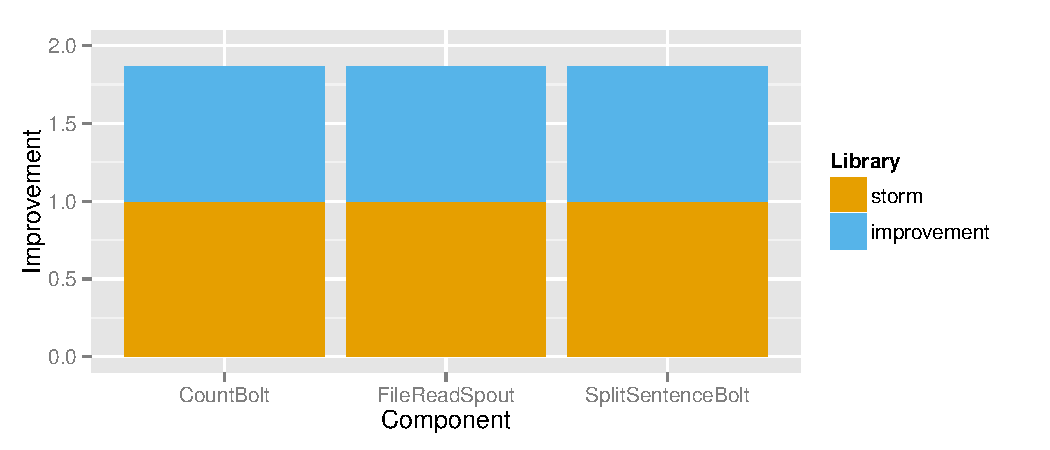
\includegraphics[width=\maxwidth]{figure/wordcount-plot-1} 

}

\caption[Improvement of Storm-MC over Apache Storm in number of tuples processed]{Improvement of Storm-MC over Apache Storm in number of tuples processed}\label{fig:wordcount-plot}
\end{figure}


\end{knitrout}


\subsection{Enron Topology}

Next, we tested the Enron topology from the IBM benchmarks. In this topology, serialised emails from the Enron email database are read from a file by a spout. They are further deserialised by one bolt, filtered by another bolt, modified by yet another bolt and then finally metrics are recorded by another bolt.

Similarly, to the WordCount topology this topology is serial in nature. However, whereas the WordCount topology keeps the random sentences in memory, the Enron topology reads from a file. Thus, this benchmark is mostly I/O intensive.

\subsection{RollingSort Topology}

The RollingSort topology is ported over from the aforementioned storm-benchmark project. This topology includes one spout and one bolt. The spout produces hundred character-long strings of random digits from zero to eight. The bolt stores a rolling window of hundred of these messages and sorts them every \textbf{x} seconds.

This benchmark is included because it is considered memory-intensive.

\todo{change x depending on the actual benchmark.}

\section{Challenges}

In this section we are going to discuss challenges we encountered while porting Apache Storm to multi-core machines.

\chapter{Conclusion}

This final chapter concludes with a summary of contributions of this project (\ref{sec:contribs}) and discusses future work that could stem from this project (\ref{sec:future_work}).

\section{Summary of Contributions}
\label{sec:contribs}

The primary contribution of this project is Storm-MC - a library aimed at data stream processing applications. The benefits of using Storm-MC are twofold:

\begin{itemize}
	\item It offers the same easy-to-use API as Apache Storm.
	\item It is tailored to multi-core environments.
\end{itemize}

Since Storm-MC uses the same API as Apache Storm, applications written with Storm in mind can be ported to use Storm-MC with minimum amount of effort. Thus if an application requires parallelism satisfiable by a single multi-core machine, it can be executed on one machine instead of a cluster.

Moreover, the Storm API allows programmers to create data stream processing applications on multi-core with an unprecedented ease. All of this comes with the superior performance Storm-MC offers compared to running Apache Storm in local mode, as shown in Section \ref{sec:performance}.

\section{Future Work}
\label{sec:future_work}

Storm-MC could be improved in a number of ways:

\begin{description}
	\item[Storm-MC as a Server] \hfill \\
	Storm-MC could be updated to enable it to run as a server. This could have several benefits such as being able to execute multiple topologies at the same time with a thin wrapper that could control their execution just like with Apache Storm. This was not implemented as we assumed most of the time users are executing only one topology per machine.
	\item[Higher Level Abstractions] \hfill \\
	Defining components of a Storm-MC topology is fairly simple. Programmers only need to define how components are connected, how they process tuples, and what tuples they emit. However, this could be taken even further with the user only specifying high-level functions and the Storm-MC library figuring out how to distribute the work. In Apache Storm this is implemented in Trident which was not ported as part of this project.
	\item[Automatic Parallelism] \hfill \\
	Sometimes when configuring a topology it may be difficult to predict the rate at which spouts are going to produce tuples. If the rate is underestimated consumers could be lagging behind producers. On the other hand, if the rate is overestimated consumers could be idle, not doing any useful work. Thus it might be advantageous to have an automatic parallelism setting which could add or remove consumers based on the current tuple rate.
	
	It may seem that this would be trivial to implement with a pool of threads representing one component. However, there are several problems that need to be considered. For example, fields grouping guarantees that tuples with the same field values go to the same executor. Changing the parallelism at runtime breaks this guarantee.
	
	Alternatively each executor could use a pool of threads. This comes with its own set of problems: the executor object would have to provide synchronised access to the pool which would only increase latency. Hence, implementing automatic parallelism was out of the scope of this project.
	\item[Performance Comparison with Distributed Storm] \hfill \\
	The benchmarks in this report compared Storm-MC to Apache Storm running in local mode. It would be interesting to see how Storm-MC compares to Apache Storm running on a cluster. One could compare the number of nodes to the number of CPUs required to execute a topology. This could provide 
\end{description}


\begin{appendices}
\chapter{Listings}
\label{ch:listings}

\begin{listing}[!htb]
\inputminted{java}{code/RandomSentenceSpout.java}
\caption{RandomSentenceSpout.java}
\label{listing:wordcount_spout}
\end{listing}

Listing \ref{listing:wordcount_spout} shows the definition of a spout that emits a randomly chosen sentence from a predefined collection of sentences.

\begin{listing}[!htb]
\inputminted{java}{code/SplitSentence.java}
\caption{SplitSentence.java}
\label{listing:wordcount_split}
\end{listing}

\begin{listing}[!htb]
\inputminted{python}{code/splitsentence.py}
\caption{splitsentence.py}
\label{listing:wordcount_split_py}
\end{listing}

Listings \ref{listing:wordcount_split} and \ref{listing:wordcount_split_py} show how a bolt defined in Python can be part of this Java-defined topology.

\begin{listing}[!htb]
\inputminted{java}{code/WordCount.java}
\caption{WordCount.java}
\label{listing:wordcount_count}
\end{listing}

Finally, listing \ref{listing:wordcount_count} shows how a bolt that counts the number of word occurrences can be implemented.


\end{appendices}

% use the following and \cite{} as above if you use BibTeX
% otherwise generate bibtem entries
\bibliographystyle{apalike}
\bibliography{mybibfile}

\end{document}
